\begin{frame}
	\frametitle{Algunos robots móviles}
	\begin{figure}[!h]
		\centering
		\subfloat[] 
		{
			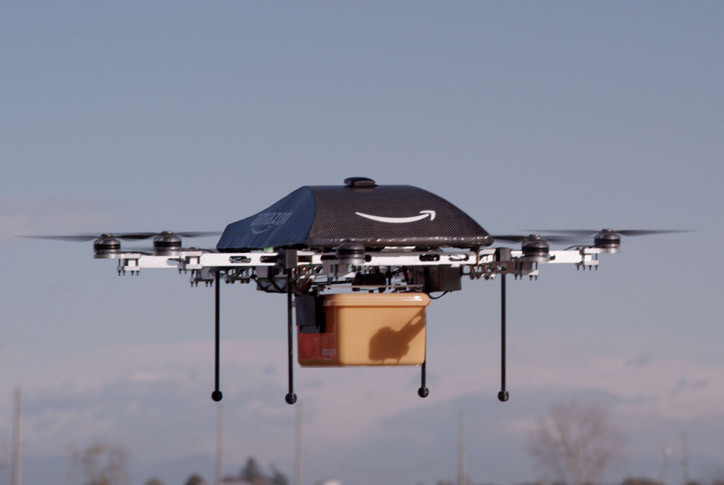
\includegraphics[width=0.33\columnwidth]{./images/introduction/drone.jpg}
		}
		\subfloat[] 
		{
			\includegraphics[width=0.33\columnwidth]{./images/introduction/GoogleCar.jpg}
		}
		\subfloat[] 
		{
			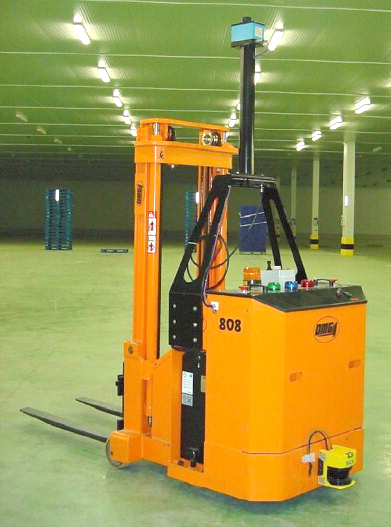
\includegraphics[width=0.16\columnwidth]{./images/introduction/industrial_robot.png}
		}\\
		\subfloat[] 
		{
			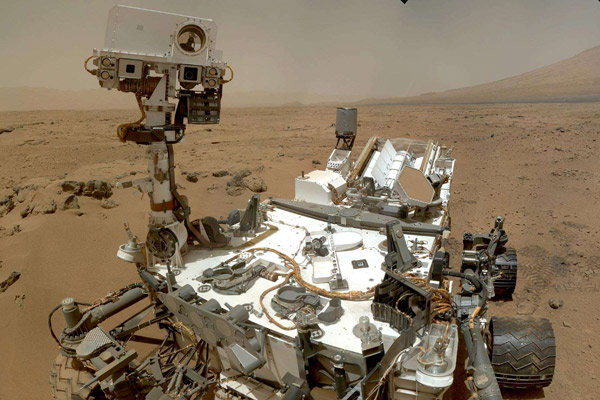
\includegraphics[width=0.33\columnwidth]{./images/introduction/curiosity.png}
		}
		\subfloat[] 
		{
			\includegraphics[width=0.33\columnwidth]{./images/introduction/hortibot.png}
		}
		\subfloat[]
		{
			\includegraphics[width=0.33\columnwidth]{./images/introduction/aqua2.png}
		}		 
	\end{figure}
\end{frame}


\begin{frame}
	\frametitle{Algunos de los sensores más utilizados}
	\begin{figure}[!h]
		\centering
		\subfloat[] 
		{
			\includegraphics[width=0.225\columnwidth]{images/introduction/telemetro.png}
		}
		\subfloat[] 
		{
			\includegraphics[width=0.15\columnwidth]{images/introduction/ir_sensor.png}
		}
		\subfloat[] 
		{
			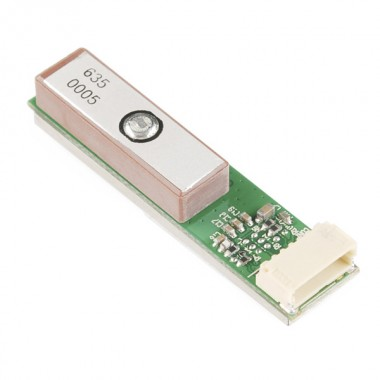
\includegraphics[width=0.18\columnwidth]{images/introduction/gps.jpg}
		}
		\subfloat[] 
		{
			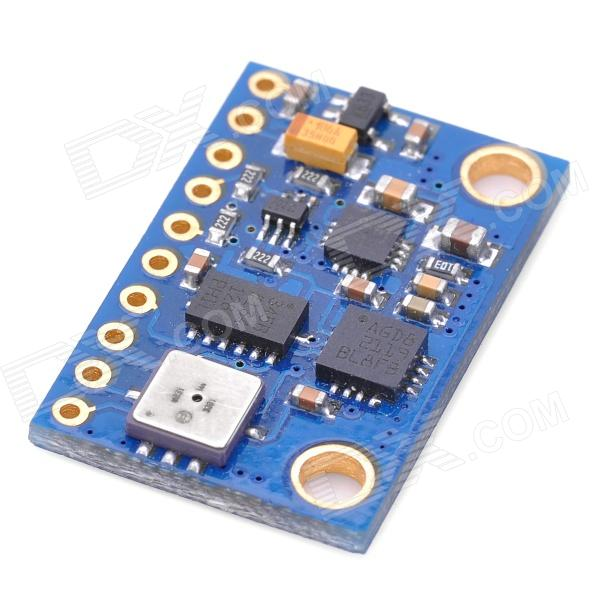
\includegraphics[width=0.18\columnwidth]{images/introduction/imu.jpg}
		}
		\subfloat[] 
		{
			\includegraphics[width=0.2\columnwidth]{images/introduction/encoders-04.jpg}
		}\\
		\subfloat[]
		{
			\includegraphics[width=0.22\columnwidth]{images/introduction/sonar.png}
		}
		\subfloat[]
		{
			\centering
			\includegraphics[width=0.3\columnwidth]{images/introduction/zed_camera2.png}
		}
		\subfloat[]
		{
			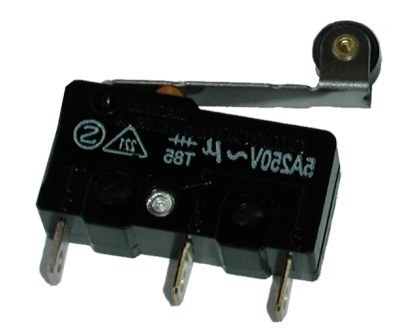
\includegraphics[width=0.16\columnwidth]{images/introduction/bumper.png}
		}
		\subfloat[]
		{
			\includegraphics[width=0.16\columnwidth]{images/introduction/laser.jpg}
		}\\
		\subfloat[]
		{
			\includegraphics[width=0.4\columnwidth]{images/introduction/xbox-360-kinect.png}
		}	
		\subfloat[]
		{
            \inlineMovie[loop]{./videos/event_camera.mp4}{images/introduction/dvs128.png}{width=0.18\columnwidth}
			%\includegraphics[width=0.16\columnwidth]{images/introduction/dvs128.png}
		}		
	\end{figure}
\end{frame}


%\begin{frame}
%	\frametitle{Algunos de las unidades de procesamiento embebido}
%	\begin{figure}[!h]
%		\centering
%		\subfigure{\includegraphics[width=0.25\columnwidth]{images/rasppi.jpg}} 
%		\subfigure{\includegraphics[width=0.4\columnwidth]{images/pc104.jpg}} 
%		\subfigure{\includegraphics[width=0.3\columnwidth]{images/arduino2560.jpg}} \\
%		\subfigure{\includegraphics[width=0.35\columnwidth]{images/placaexabot.png}}
%		\subfigure{\includegraphics[width=0.3\columnwidth]{images/driver.jpg}}  
%		\subfigure{\includegraphics[width=0.28\columnwidth]{images/arduinoVR.jpg}}
%		%\subfigure{\includegraphics[width=0.28\columnwidth]{images/driverPP.jpg}}
%		
%	\end{figure}
%\end{frame}



\begin{frame}
	\frametitle{Navegación autónoma}
	\begin{block}{}
		La navegación autónoma puede definirse a grandes rasgos como la capacidad de moverse de forma segura a lo largo de una trayectoria entre un punto de inicio y uno final [1].
	\end{block}
	\vspace{5mm}
	\begin{columns}
		\column{0.4\textwidth}
		\hspace{13pt}Pregunta:
		\begin{enumerate}
			\visible<2-7>{ \item[-] ¿Dónde estoy?}
			\visible<4-7>{\item[-] ¿Por dónde estoy yendo?}
			\visible<6-7>{\item[-] ¿Cómo llego hasta allí?}
		\end{enumerate}
		\column{0.6\textwidth}
		Respuesta:
		\begin{enumerate}[$\rightarrow$]
			\visible<3-7>{ \item  Cálculo de la posición (Localization)}
			\visible<5-7>{ \item  Representación del entorno (Mapping)}
			\visible<7-7>{\item  Planeamiento de movimiento (Motion planning)}
		\end{enumerate}
	\end{columns}
	\only<4>{}
	\vfill
	\begin{tiny}
		[1] J. J. Leonard - et al., ``Mobile robot localization by ...,'' IEEE Transactions on Robotics and Automation, 2002.
	\end{tiny}
\end{frame}
